\newcommand{\decktitle}{Editoren \& IDEs}

%%%%%%%%%%%%%%%%%%%%%%%%%%%%%%%%%%%%%%%%%%%%%%%%%
%
% DOCUMENT
%
%%%%%%%%%%%%%%%%%%%%%%%%%%%%%%%%%%%%%%%%%%%%%%%%%

\begin{frame}
    \subtitle{\decktitle}
    \titlepage
\end{frame}


\begin{frame}
    \frametitle{\textbf{Outline:}}
    \tableofcontents
\end{frame}

		
\section{Code-Editoren \& IDEs}

  \begin{frame}{Ausführungsarten von Python-Code (I)}
      Wie bereits beschrieben kann Python-Code auf unterschiedliche Arten und Weisen ausgeführt werden. \\~\
      
      Eine Möglichkeit besteht darin, den Code direkt in den Python-Interpreter einzugeben. Hierdurch wird der Code sofort und unmittelbar ausgeführt, was insbesondere dann hilfreich ist, wenn schnell eine gewisse Funktionalität ausprobiert werden soll. \\~\
      
      Der Nachteil besteht jedoch darin, dass der Code, der direkt im Python-Interpreter eingegeben wird, nicht persistiert wird. Das bedeutet, dass der Code nicht abgespeichert wird, sobald der Interpreter geschlossen wird ist der Code verloren. Zudem kann der Code auf diese Weise nicht mit anderen Mitbearbeitern geteilt werden, der Code kann schlecht strukturiert werden, etc...
  \end{frame}
  
    \begin{frame}{Ausführungsarten von Python-Code (II)}
      Um diese Nachteile zu umgehen, bietet es sich an, den Code in Python-Dateien zu speichern und diese Dateien dann auszuführen. So wird die Arbeit mit dem Python-Code deutlich einfacher, übersichtlicher und strukturierter. \\~\
      
      Der Code innerhalb der Dateien kann ausgeführt werden, indem dem Python-Interpreter der Dateipfad angehangen wird, in der der Code gespeichert ist. \\~\
      
      Ist der Code also beispielsweise in der Datei \code{main.py} gespeichert, kann der Code ausgeführt werden mit \code{python main.py} (sofern man sich im gleichen Verzeichnis wie die entspr. Datei befindet). \\~\
      
      Alternativ kann auch ein absoluter Pfad übergeben werden, z.B. \code{python C:\textbackslash{}Users\textbackslash{}Jonas\textbackslash{}Programming\textbackslash{}main.py} (unabhängig vom aktuellen Pfad)
      
  \end{frame}
  
  \begin{frame}{Ausführuhngsarten von Python-Code (III)}
      \begin{alertblock}{Interpreter- vs. Datei-Modus}
        Wird lediglich der Befehl \code{python} ausgeführt, wird der Python Interpreter gestartet, während durch den Befehl \code{python datei.py} der Code aus der entsprechenden Datei ausgelesen wird und dem Interpreter zur Ausführung übergeben wird. Auf diese Weise gelangt man also nicht in den interaktiven ausführbaren Modus.
      \end{alertblock}
  \end{frame}
  
    \begin{frame}{Ausführuhngsarten von Python-Code (IV)}
      \begin{block}{Python Dateiendung}
        Dateien, in denen Python-Code gespeichert ist, werden i.d.R. mit der Dateiendung \code{.py} abgespeichert, damit offensichtlich ist, dass es sich dabei um Python-Dateien handelt (analog zu bspw. \code{.jpg} für Bilder oder \code{.txt} für Textdateien). \\~\
        
        Die Dateiendung \code{.py} ist nicht zwingend notwendig, jedoch Best Practice bzw. Teil der Konvention und sollte daher immer genutzt werden.
      \end{block}
  \end{frame}
  
  \begin{frame}{Code-Editoren}
      Python-Code, der in Dateien gespeichert wird, kann mithilfe jeden beliebigen Text-Editor geschrieben werden, bspw. den standardmäßig vorinstallierten \textit{Windows Editor} auf Windows-Systemen oder auch \textit{TextEdit} auf macOS.\\~\
      
      Dennoch sind diese simplen Texteditoren kaum dafür geeignet, Code zu verfassen, da sie keinerlei Hilfestellungen oder anderweitige Features bieten, die dabei helfen, fehlerfreien und sauberen Code zu schreiben. \\~\
      
      Daher gibt es spezielle Code-Editoren, die als Text-Editoren mit derartigen Funktionen gesehen werden können.
  \end{frame}
  
  \begin{frame}{Features von Code-Editoren}
      Code-Editoren bieten beispielsweise folgende Features:
      
      \begin{itemize}
          \item Code- / Syntax-Highlighting (unterschiedliche Farben für unterschiedliche Programm-Bestandteile (Variablen, Funktionsdefinitionen, Schlüsselwörter, ...))
          \item Autovervollständigung: Schlüsselwörter oder bereits zuvor deklarierte Variablennamen können vervollständigt werden
          \item Einrückung: Code kann korrekt eingerückt werden, keine Vermischung von Tabulator- und Leerzeichen
          \item Hervorheben von zusammengehörigen Blöcken: Der Bereich von if-Clauses, Schleifen oder Funktionen wird gekennzeichnet
          \item ...
      \end{itemize}
      
      Code-Editoren können also dazu beitragen, Fehler frühzeitig zu erkennen und zu beheben sowie die Produktivität des Entwicklers und Qualität des Codes zu steigern.
  \end{frame}
  
  \begin{frame}{Bekannte Code-Editoren}
      Es gibt eine Vielzahl an Code-Editoren, die genutzt werden können. Viele davon sind kostenlos und quelloffen.\\~\
      
\begin{itemize}
    \item \href{https://code.visualstudio.com/}{Visual Studio Code}
    \item \href{https://www.sublimetext.com/}{Sublime Text 3}
    \item \href{https://atom.io/}{Atom text editor}
    \item \href{https://notepad-plus-plus.org/}{Notepad++} (nur Windows)
    \item \href{https://macromates.com/}{TextMate} (nur macOS)
\end{itemize}
  \end{frame}
  
  \begin{frame}{Integrierte Entwicklungsumgebungen (IDEs)}
      Neben Code-Editoren existieren auch sogenannte \textit{Integrierte Entwicklungsumgebungen} (engl. \textit{Integrated Development Environments (IDEs)}). \\~\
      
      Diese bieten im Vergleich zu "einfachen" Code-Editoren erweiterte Funktionalitäten wie z.B.
      
      \begin{itemize}
          \item integrierte Versionsverwaltung
          \item integrierte Compiler / Interpreter / Linker
          \item Werkzeuge zur Steigerung der Produktivität
          \item Tools zur Unterstützung bei der Entwicklung graphischer Benutzeroberflächen
          \item ...
      \end{itemize}
        
  \end{frame}
  
   \begin{frame}{Bekannte IDEs}
      Im professionellen Umfeld werden zur Code-Entwicklung meist IDEs verwendet. Aufgrund des großen Funktionsumfangs sind IDEs häufig kostenpflichtig.
      
      \begin{itemize}
          \item \href{https://www.jetbrains.com/de-de/pycharm/}{PyCharm}
          \item \href{https://www.eclipse.org/}{Eclipse}
          \item \href{https://www.spyder-ide.org/}{Spyder}
          \item \href{https://docs.python.org/3/library/idle.html}{IDLE} (enthalten in der Standard Python Installation
          \item \href{https://code.visualstudio.com/}{Visual Studio Code}
      \end{itemize}
        
  \end{frame}
  
\section{Visual Studio Code}

    \begin{frame}{Visual Studio Code}
        In dieser Veranstaltung werden Übungen und Codebeispiele mithilfe von Visual Studio Code (kurz: VS Code) umgesetzt. \\~\
        
        VS Code ist eine Mischung aus Code-Editor und IDE und wird von Microsoft entwickelt. Das Programm ist plattformunabhängig und kann auf Windows, macOS und anderen Systemen ausgeführt werden. \\~\
        
        VS Code kann unter \href{https://code.visualstudio.com/}{https://code.visualstudio.com/} heruntergeladen werden.
        
        \begin{block}{Wahl des Code-Editors}
            Die Studierenden können ein beliebiges Programm ihrer Wahl zur Programmierung nutzen. Es wird aber empfohlen VS Code zu nutzen, da hierfür die beste Hilfestellung gegeben werden kann.
        \end{block}
    \end{frame}
    
    \begin{frame}{Visual Studio Code - Einrichtung (I)}
        Nach der Installation von VS Code und dem Öffnen des Programms sollte Folgendes zu sehen sein:
        
        \begin{figure}
            \centering
            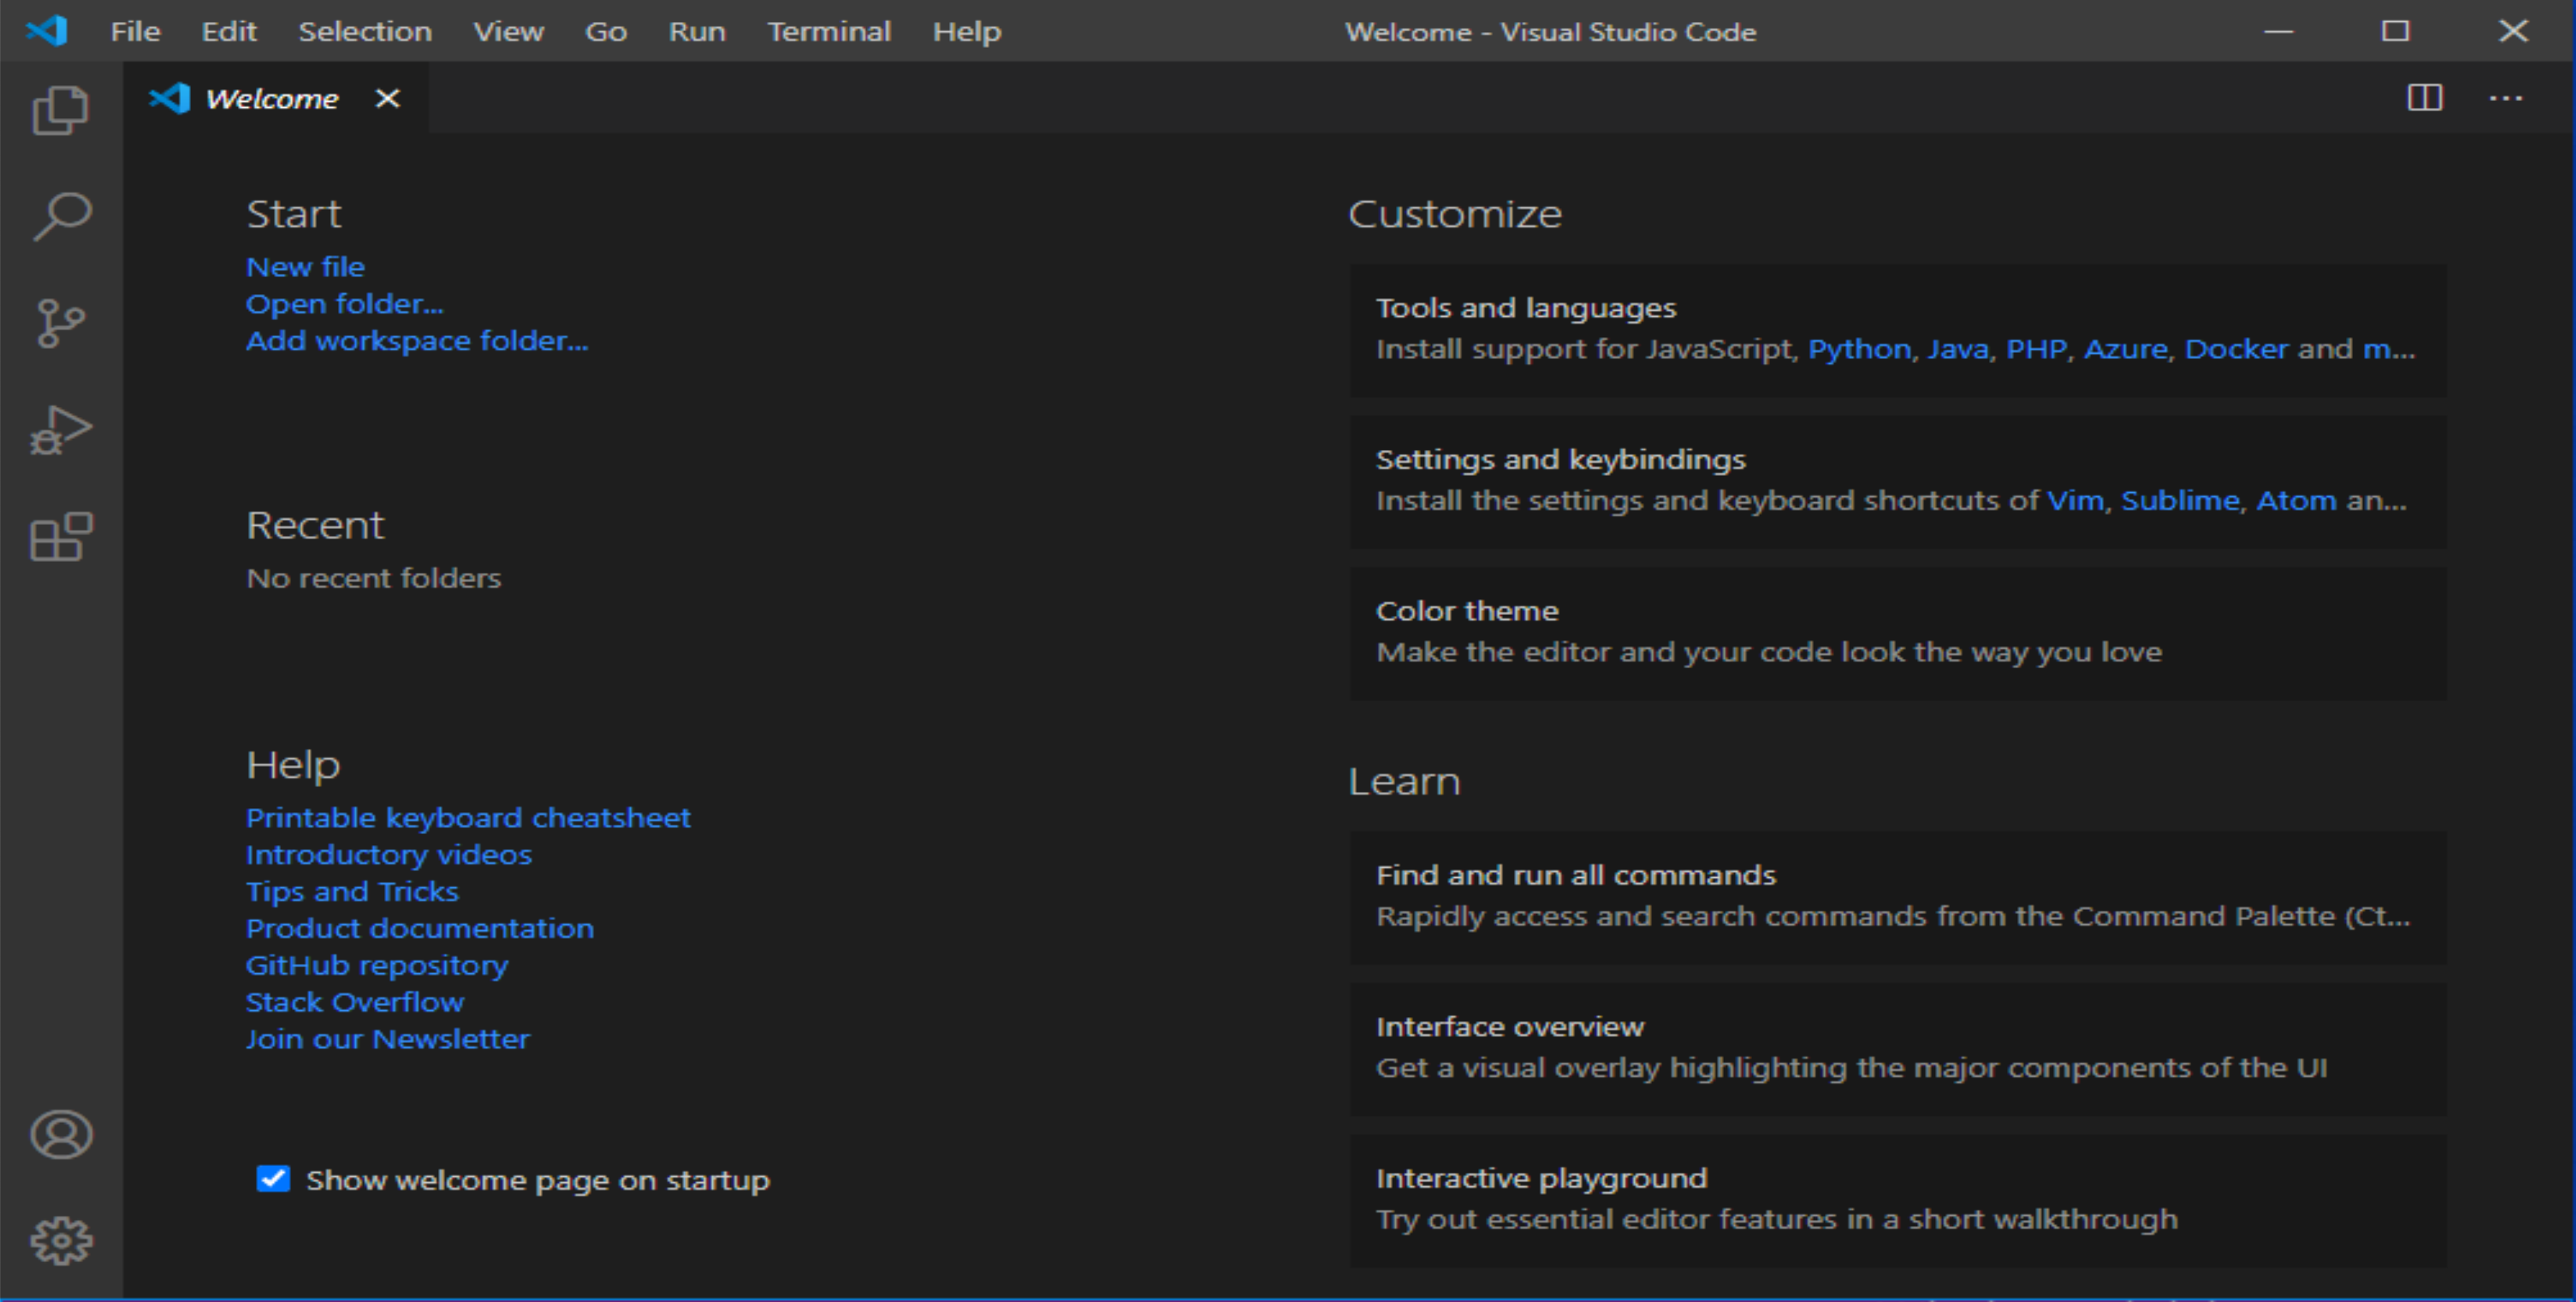
\includegraphics[keepaspectratio, width=0.9\linewidth]{chapters/08_ide/figures/vs_code_start.png}
            \caption{VS Code nach dem 1. Start}
        \end{figure}
    \end{frame}
    
    \begin{frame}{Visual Studio Code - Einrichtung (II)}
        Die Bearbeitung von Projekten/Dateien erfolgt in VS Code Workspacebasiert, d.h. es wird ein bestimmter Ordner als Workspace bestimmt, innerhalb dessen die Dateien verwaltet werden.\\~\
        
        Ein Workspace kann angelegt werden, indem direkt auf der Startseite \code{Add workspace folder...} oder unter \code{File} der Menüpunkt \code{Open Workspace...} ausgewählt wird.\\~\
        
        Hier bietet es sich an, einen Ordner zu erstellen, in dem alle Übungen und Codebeispiele gespeichert werden. Dieser Ordner dient dann als Workspace.
    \end{frame}
    
    \begin{frame}{Visual Studio Code - Einrichtung (III)}
        Nachdem der Workspace angelegt wurde, steht dieser zur Arbeit bereit. In der linken Leiste von VS Code gibt es verschiedene Reiter, der erste Reiter zeigt die Datei-/Ordnerstruktur des aktuellen Workspaces an. \\~\
        
        Durch einen Rechtsklick können so neue Ordner und Dateien angelegt werden
        
        \begin{figure}
            \centering
            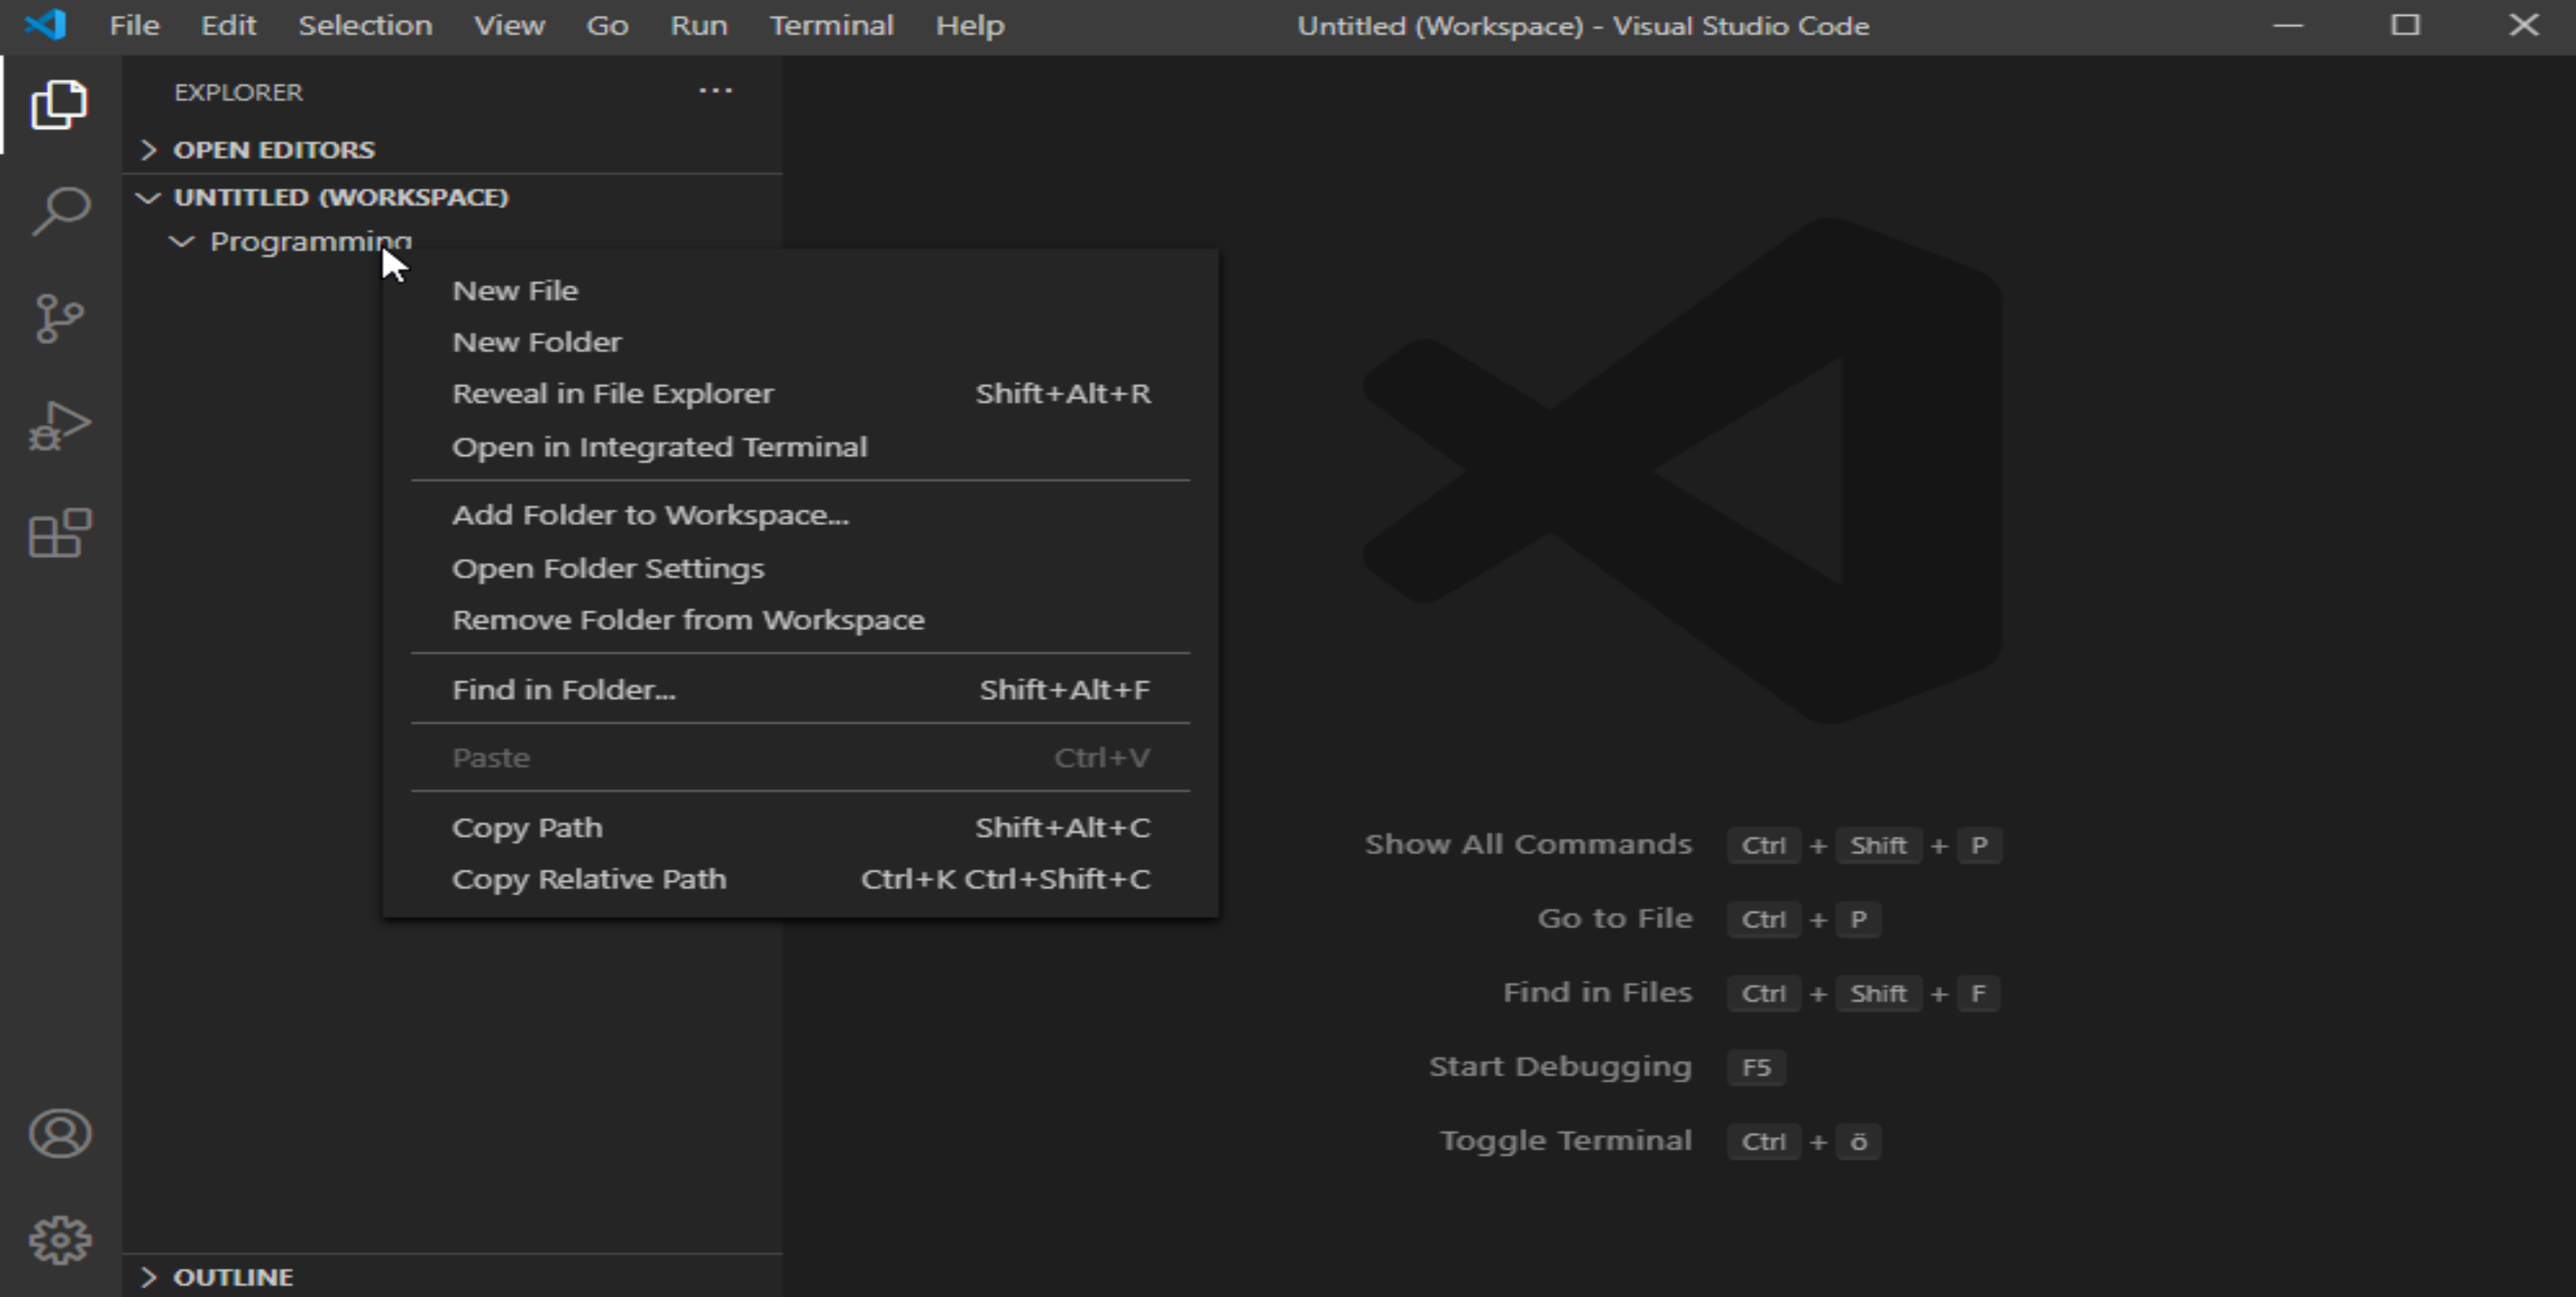
\includegraphics[keepaspectratio, width=0.9\linewidth]{chapters/08_ide/figures/vs_code_create_file.png}
            \caption{Anlegen einer neuen Datei oder Verzeichnisses}
        \end{figure}
    \end{frame}
    
     \begin{frame}{Visual Studio Code - Einrichtung (IV)}
        Wird eine neue \code{.py}-Datei angelegt, erkennt VS Code, dass es sich dabei um eine Python-Datei handelt und schlägt automatisch die Python-Erweiterung vor. Es wird empfohlen, diese zu installieren, um Python-spezifische Features zu aktivieren.
        
        \begin{figure}
            \centering
            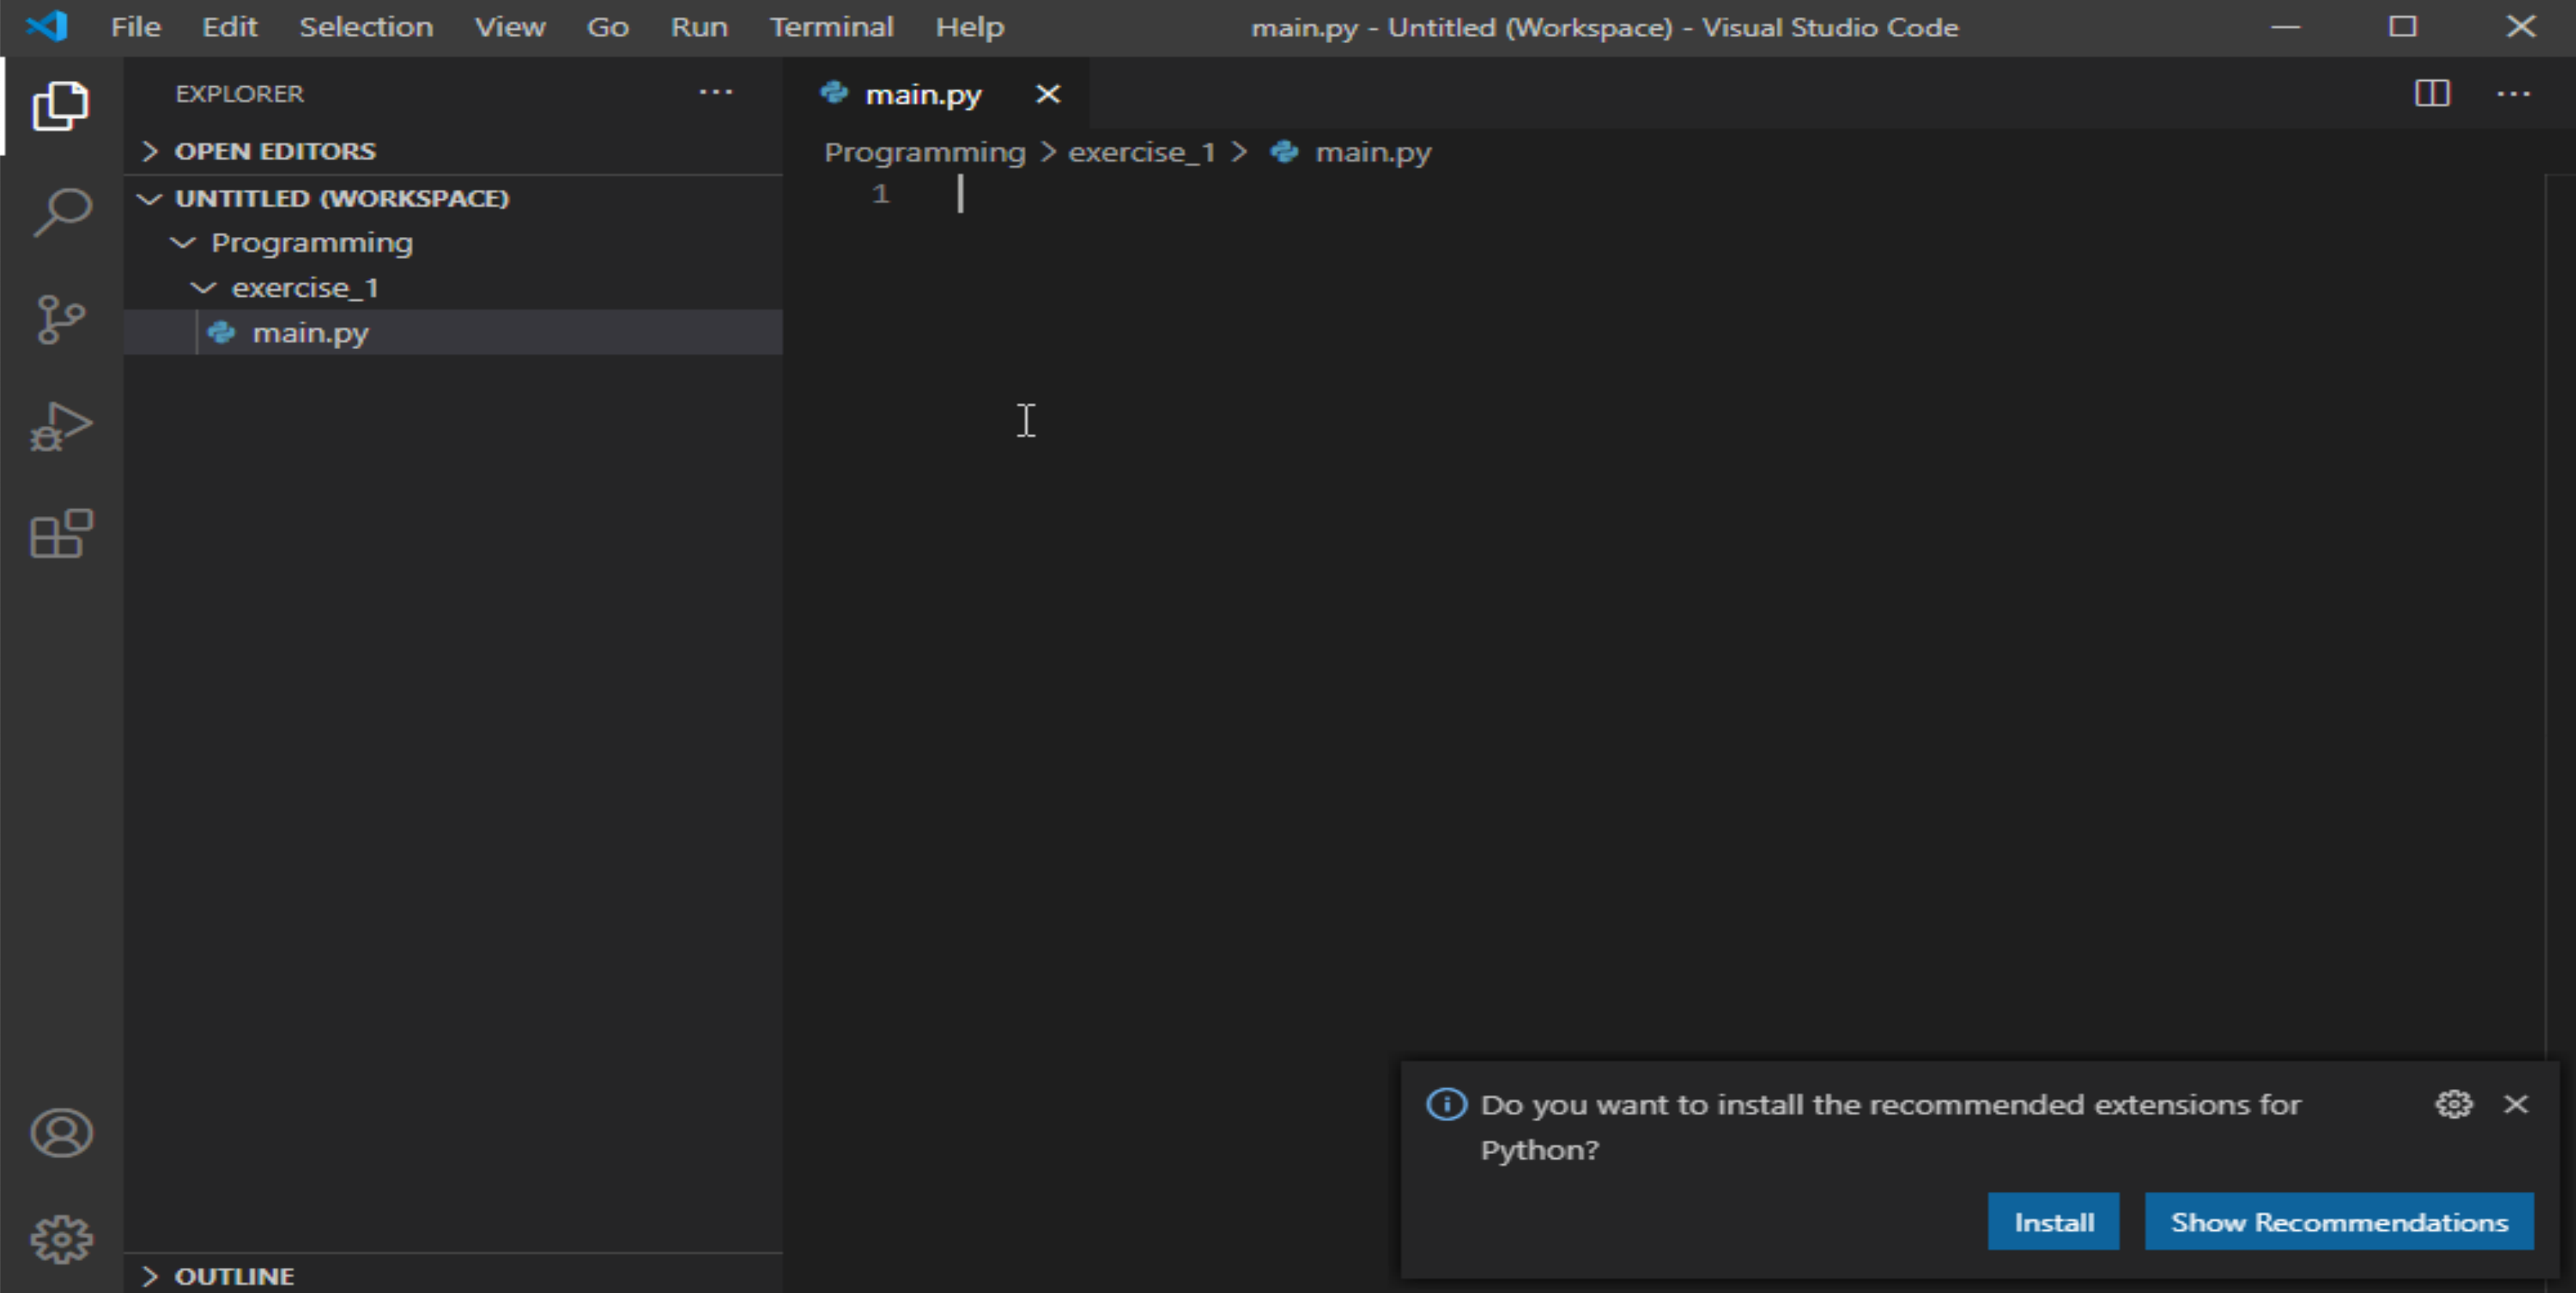
\includegraphics[keepaspectratio, width=0.9\linewidth]{chapters/08_ide/figures/vs_code_python.png}
            \caption{Vorschlag zur Installation der Python-Erweiterung}
        \end{figure}
        
    \end{frame}
    
    \begin{frame}{Visual Studio Code - Einrichtung (V)}
        Sobald die Python-Erweiterung installiert ist, wird automatisch ein installierter Python-Interpreter gesucht und links unten in der unteren Programmleiste angezeigt. Stellen Sie sicher, dass hier der korrekte Interpreter ausgewählt ist
        
        \begin{figure}
            \centering
            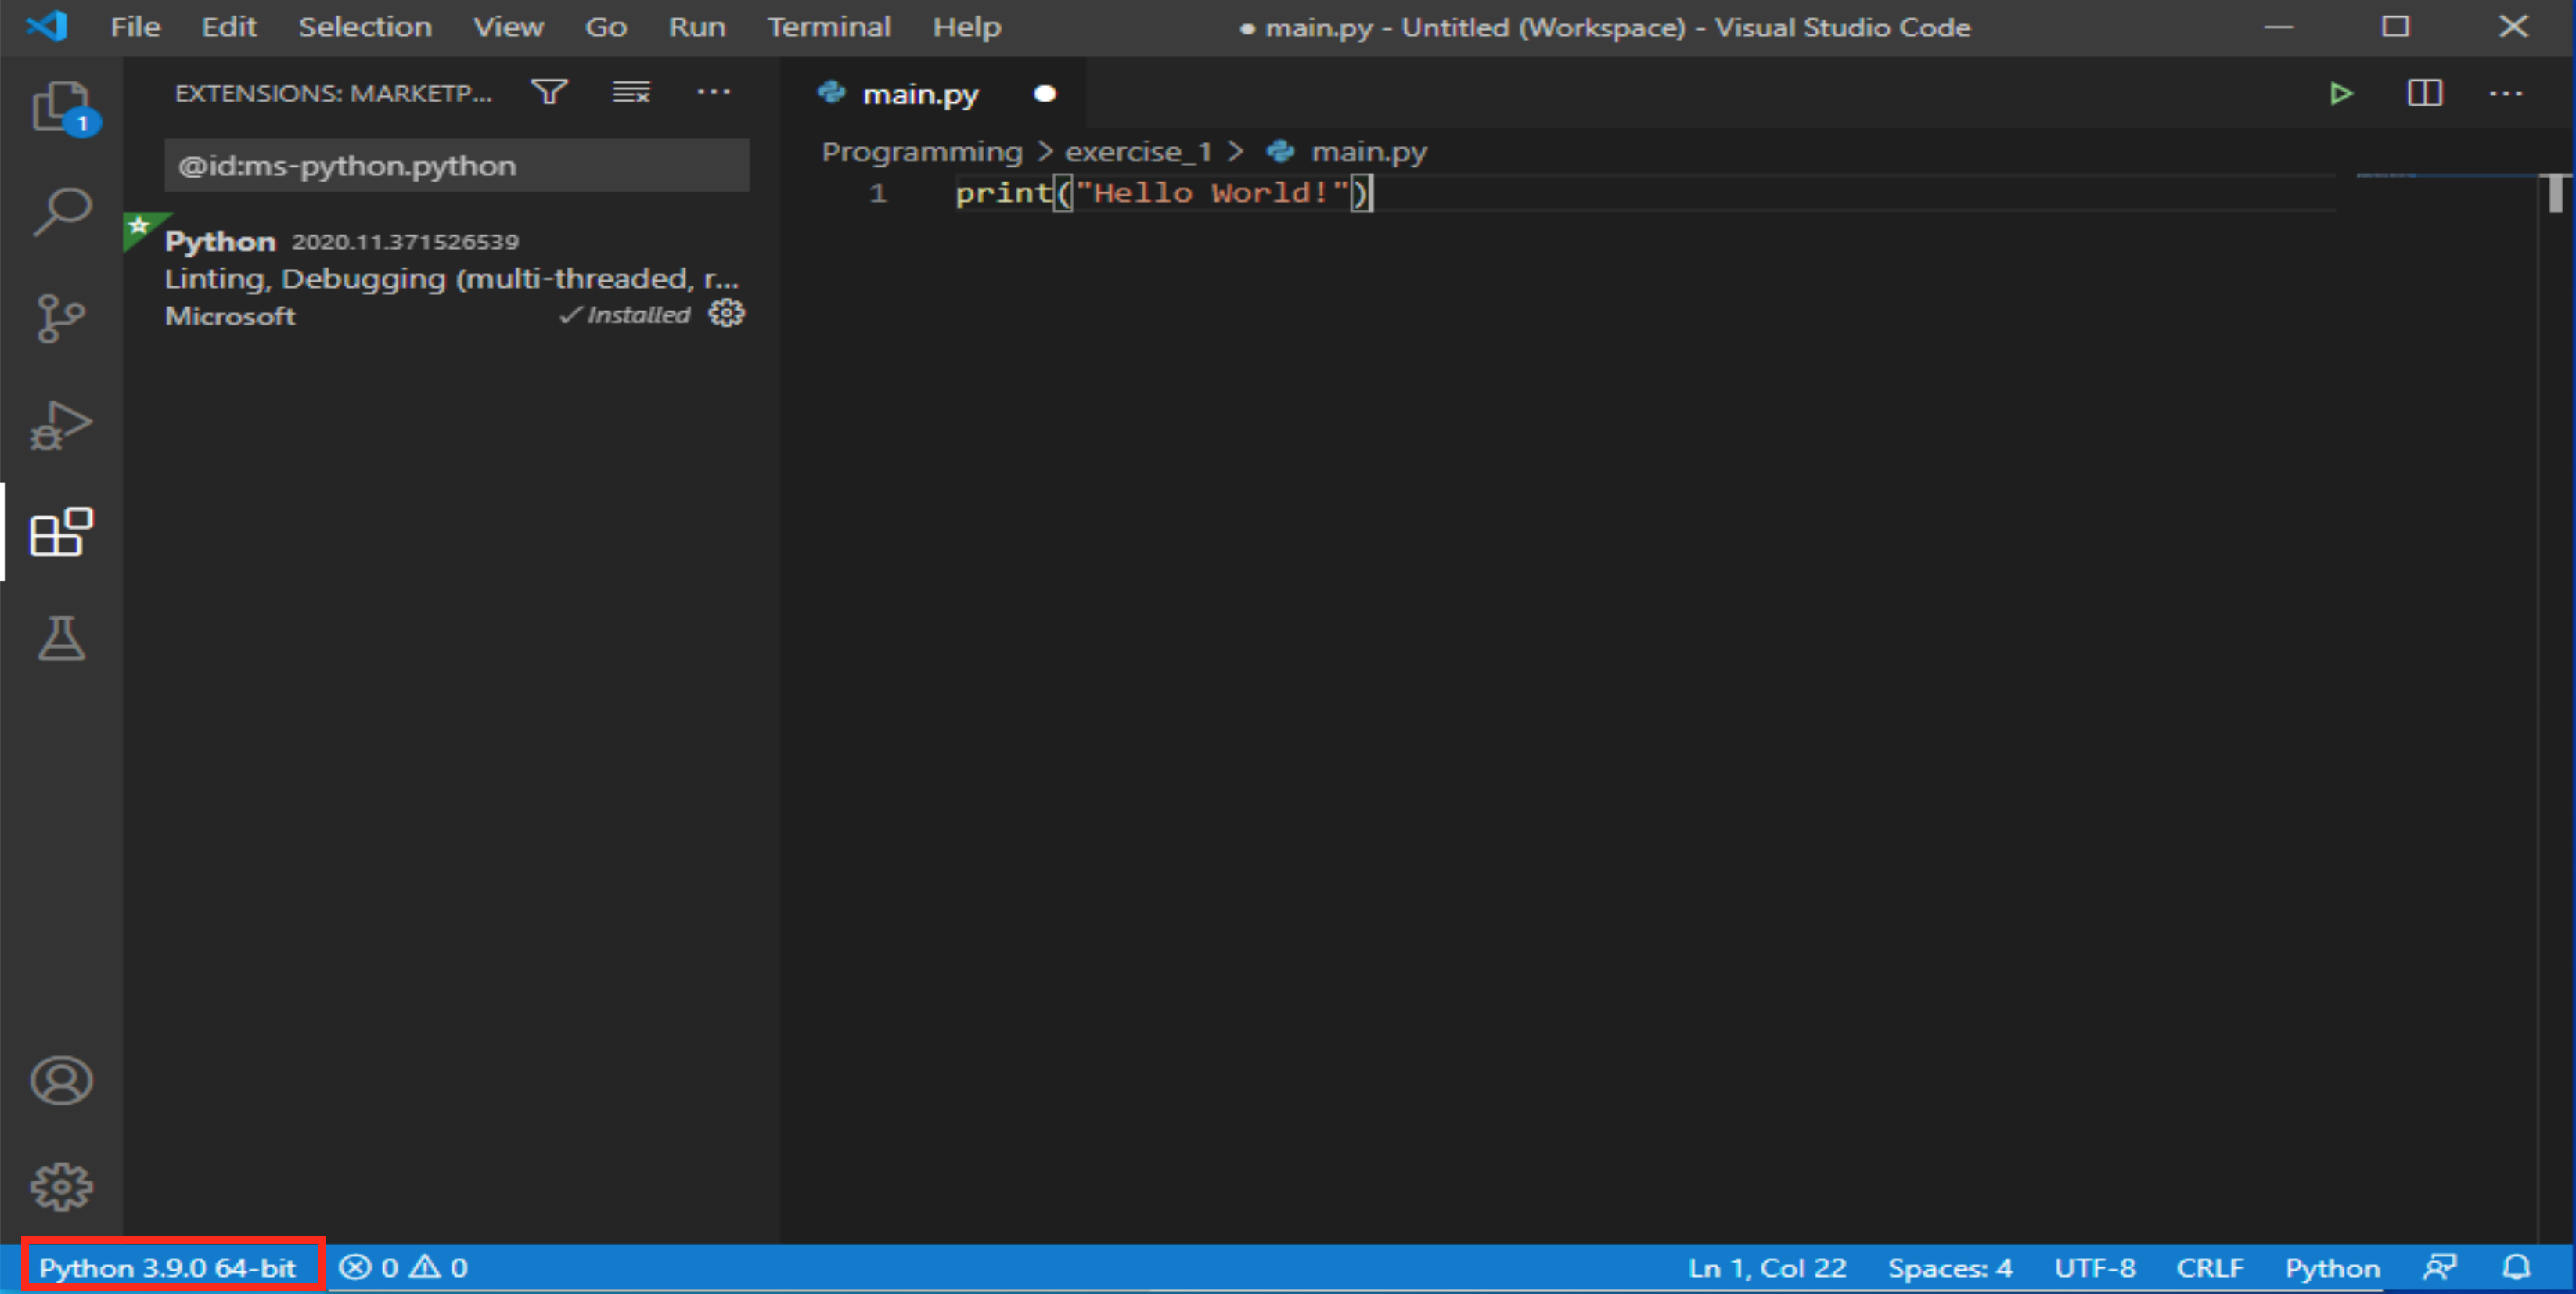
\includegraphics[keepaspectratio, width=0.9\linewidth]{chapters/08_ide/figures/vs_code_python_interpreter.png}
            \caption{Anzeige des aktuell verwendeten Python Interpreters}
        \end{figure}
        
    \end{frame}
    
        \begin{frame}{Visual Studio Code - Einrichtung (VI)}
        Wird nun eine Python Datei geöffnet, so kann diese direkt aus dem Editor heraus ausgeführt werden, indem das grüne Dreieck im oberen rechten Bereich gedrückt wird. Hierdurch wird die Konsole im unteren Bereich geöffnet, in der die Ausgabe erfolgt.
        
        \begin{figure}
            \centering
            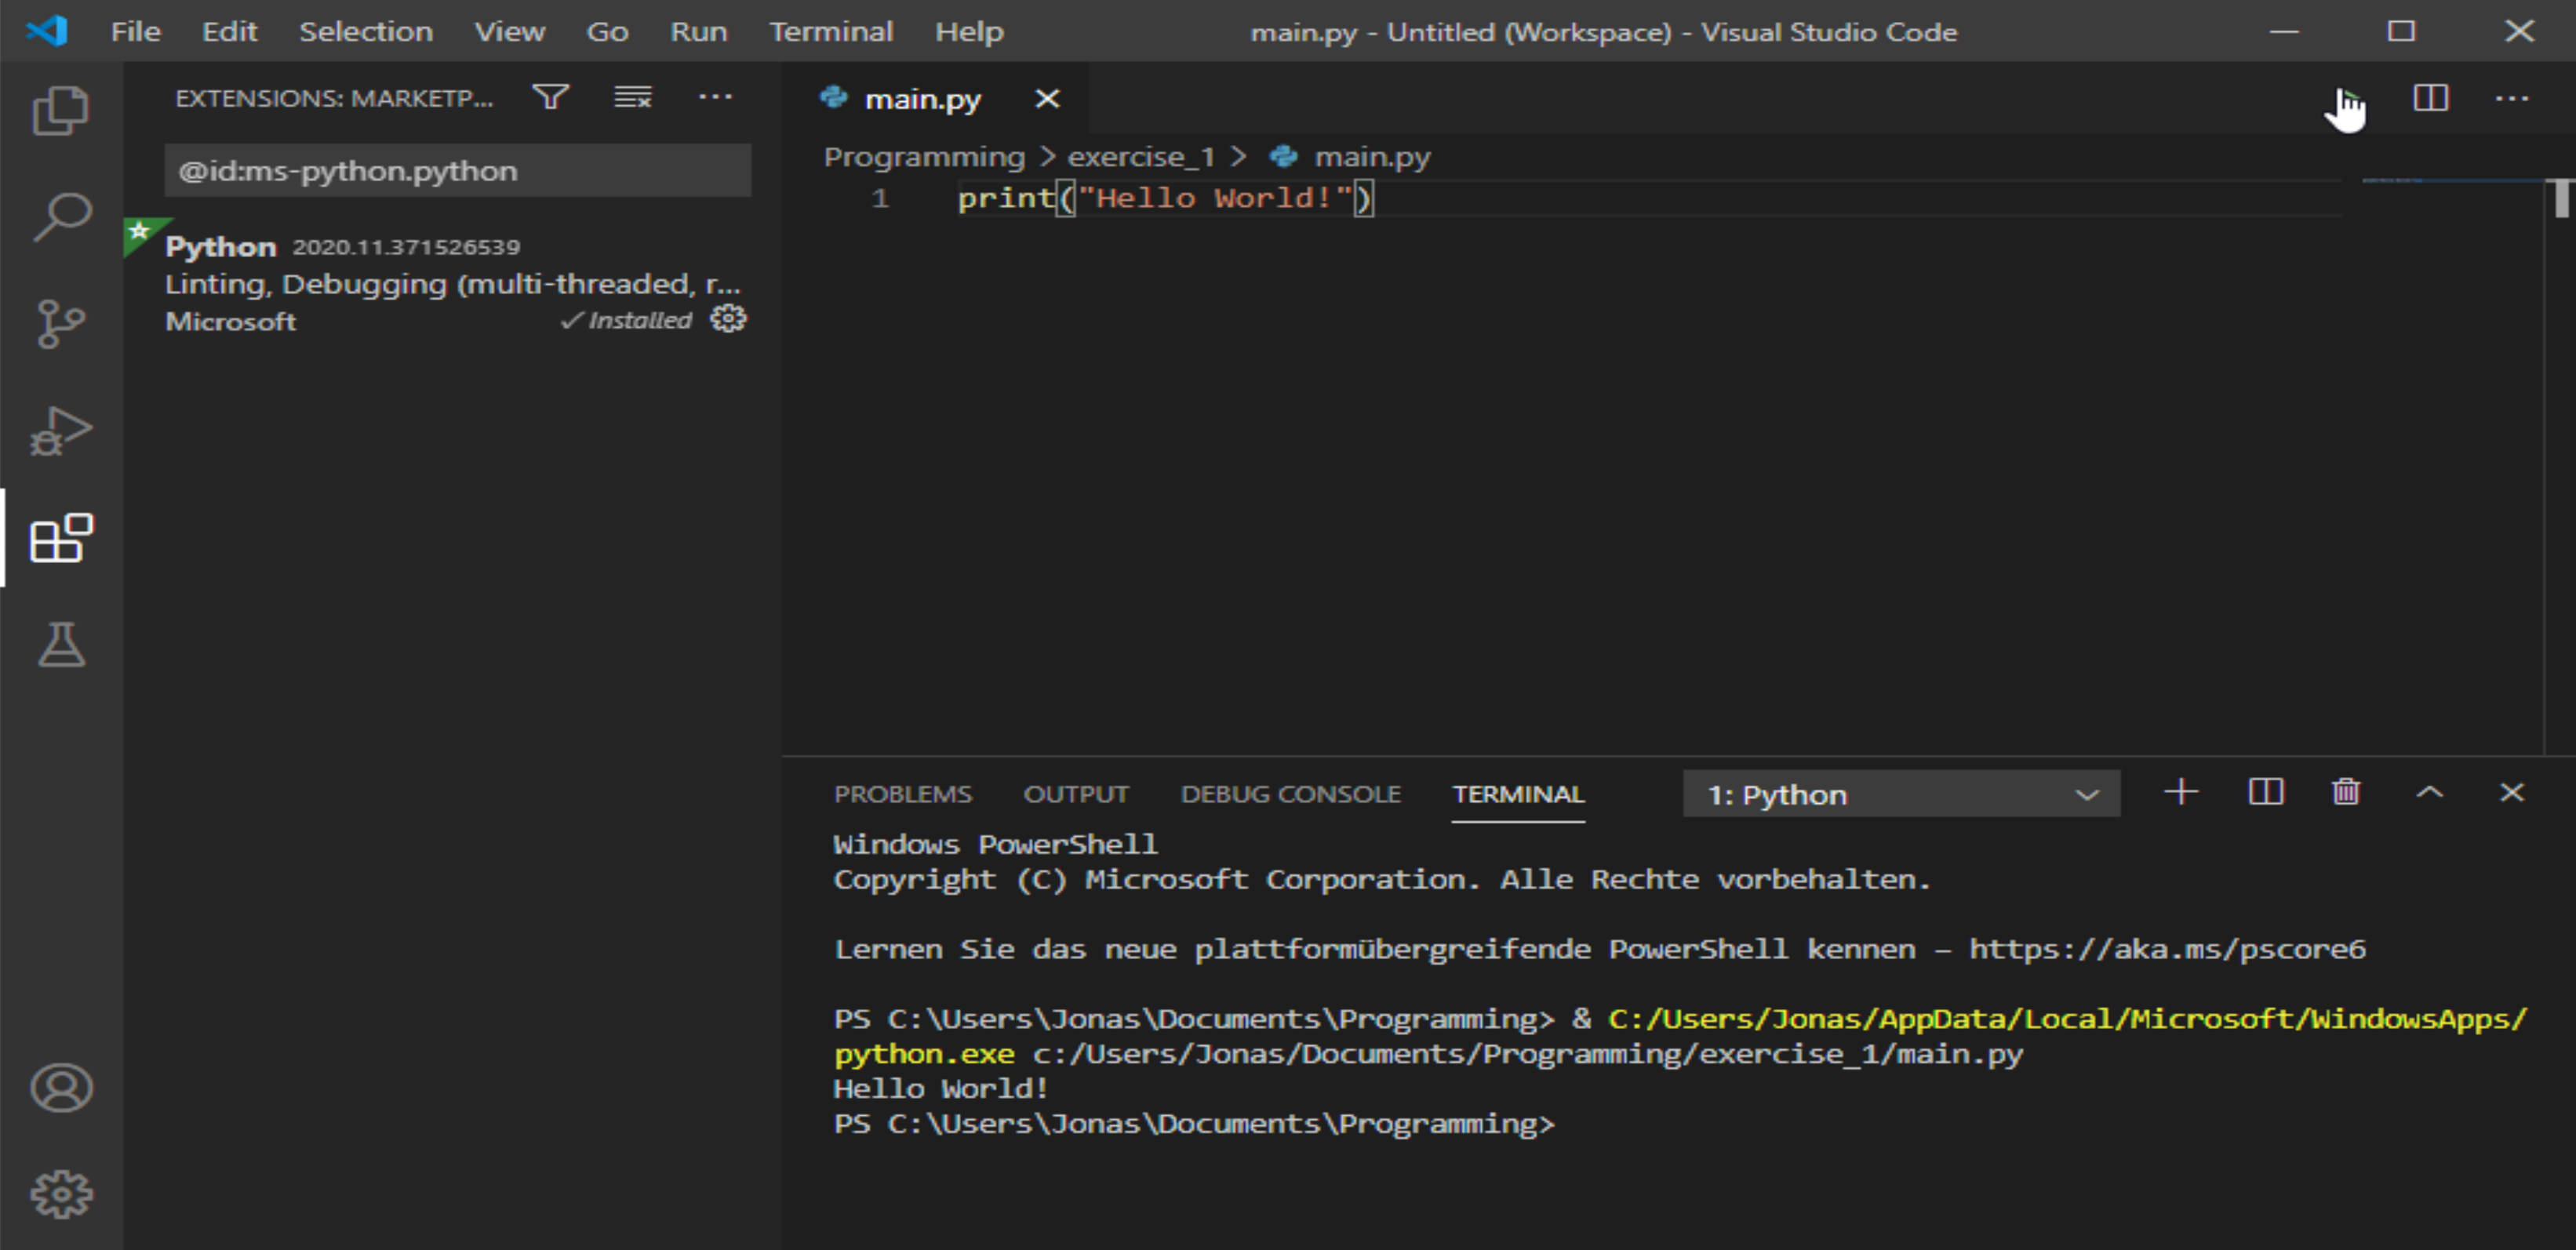
\includegraphics[keepaspectratio, width=0.9\linewidth]{chapters/08_ide/figures/vs_code_python_run.png}
            \caption{Ausführen der Python Datei}
        \end{figure}
        
    \end{frame}
    
    \begin{frame}{Visual Studio Code - Einrichtung (VII)}
        Achtung: Wird hinter dem Dateinamen ein weißer Punkt angezeigt, bedeutet das, dass die Änderungen in der Datei noch nicht gespeichert wurden.
        
        \begin{figure}
            \centering
            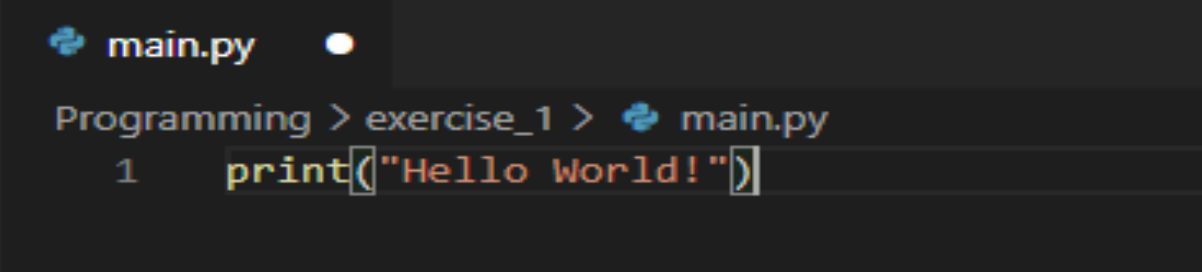
\includegraphics[keepaspectratio, width=0.9\linewidth]{chapters/08_ide/figures/vs_code_not_saved.png}
            \caption{Ungespeicherte Änderungen in der Datei main.py}
        \end{figure}
        
    \end{frame}